\chapter{Marco Teórico} \label{Marco Teorico}

En este capítulo se hará una revisión de conceptos básicos de la ingeniería dirigida por modelos, perfiles UML y diagramas de deployment. Se introducirá el concepto de sistema de manejo de la configuración, junto con algunos ejemplos de los mismos, y se mostrarán ejemplos de herramientas de simulación y visualización de redes, relacionadas a la temática. Finalmente se encontrará una breve introducción a herramientas de modelado, en particular Eclipse Modeling Tools, y algunos ejemplos de MDE aplicado a redes de computadoras.

\section{Estado del Arte}
\subsection{Herramientas de simulación de redes de computadoras} \label{Herramientas de simulación}
\subsubsection{M5 Simulator}
La herramienta de código abierto M5 Simulator es utilizada para permitir la investigación en redes TCP/IP. Provee las características necesarias para simular redes de hosts, incluyendo todas las funcionalidades de un sistema, un detallado sistema de I/O, y la capacidad de simular múltiples sistemas en red.
Se describe como un simulador de arquitecturas de propósito general, con un enfoque hacia networking. \cite{binkert2006m5}

Si bien esta herramienta es capaz de simular redes, no provee un editor gráfico para realizar diagramas de las mismas, lo mismo sucede con las herramientas de generación de topologías que se verán a continuación.
\subsection{Herramientas de generación de topologías de red}
Existen varias herramientas para la generación de topologías de red, que permiten hacer simulaciones sobre las topologías generadas. Estas herramientas, sin embargo, están enfocadas en la estructura de la topología, y por lo tanto, se basan en la generación de nodos y su estructura a un alto nivel, por lo que no son utilizadas para diferenciar dispositivos de red en particular.
Hay diferentes clases de generadores, en base a la forma en que generan los grafos, dos de los más conocidos son los siguientes \cite{tangmunarunkit2002network}:
\begin{description}
\item[Tiers:] es un generador \textit{estructural}, esta herramienta se enfoca en generar topologías multinivel (multi-tier), e implementa simulación de modelos que imitan la estructura de red de internet.

\item[Waxman:] este generador es de la clase de \textit{grafos aleatorios}, genera grafos aleatorios en base al modelo de Erdos-Renyi, que asigna una probabilidad uniforme para crear una conexión entre cada par de nodos. Waxman extiende este modelo asignando los nodos, de forma aleatoria, a posiciones en un plano, y basando la probabilidad de creación de conexión entre un par nodos en la distancia que existe entre ellos. 
\end{description}

\subsection{Herramientas de visualización de redes de computadoras} \label{Herramientas de visualización}
\subsubsection{SolarWinds: Network Topology Mapper \cite{solarwinds}} \label{SolarWinds Topology Mapper}
SolarWinds es una herramienta utilizada para escanear y mapear la infraestructura de la red, incluyendo dispositivos de red, servidores, y hosts virtualizados.
Algunas de sus características principales son:
\begin{itemize}
\item La capacidad de detectar y delinear automáticamente la topología de la red, y generar diagramas de red completos. 
\item Ofrece la posibilidad de elegir diferentes métodos de detección. \item Permite exportar los diagramas en diferentes formatos.
\item Brinda informes robustos sobre puertos de conmutación, VLAN, subredes e inventario.
\item Aborda directamente el cumplimiento con PCI, FIPS 140-2, etc. que requieren mantenimiento de un diagrama de red actualizado.
\end{itemize}

En la Figura \ref{fig:marco:solarwinds} se puede ver un ejemplo de un diagrama de red creado utilizando la herramienta.
Es importante notar que esta herramienta se basa en la detección y generación de diagramas de red, sin embargo, no ofrece la posibilidad de generar archivos de configuración a partir de estos diagramas.

\begin{figure}[htbp]
    \centering
    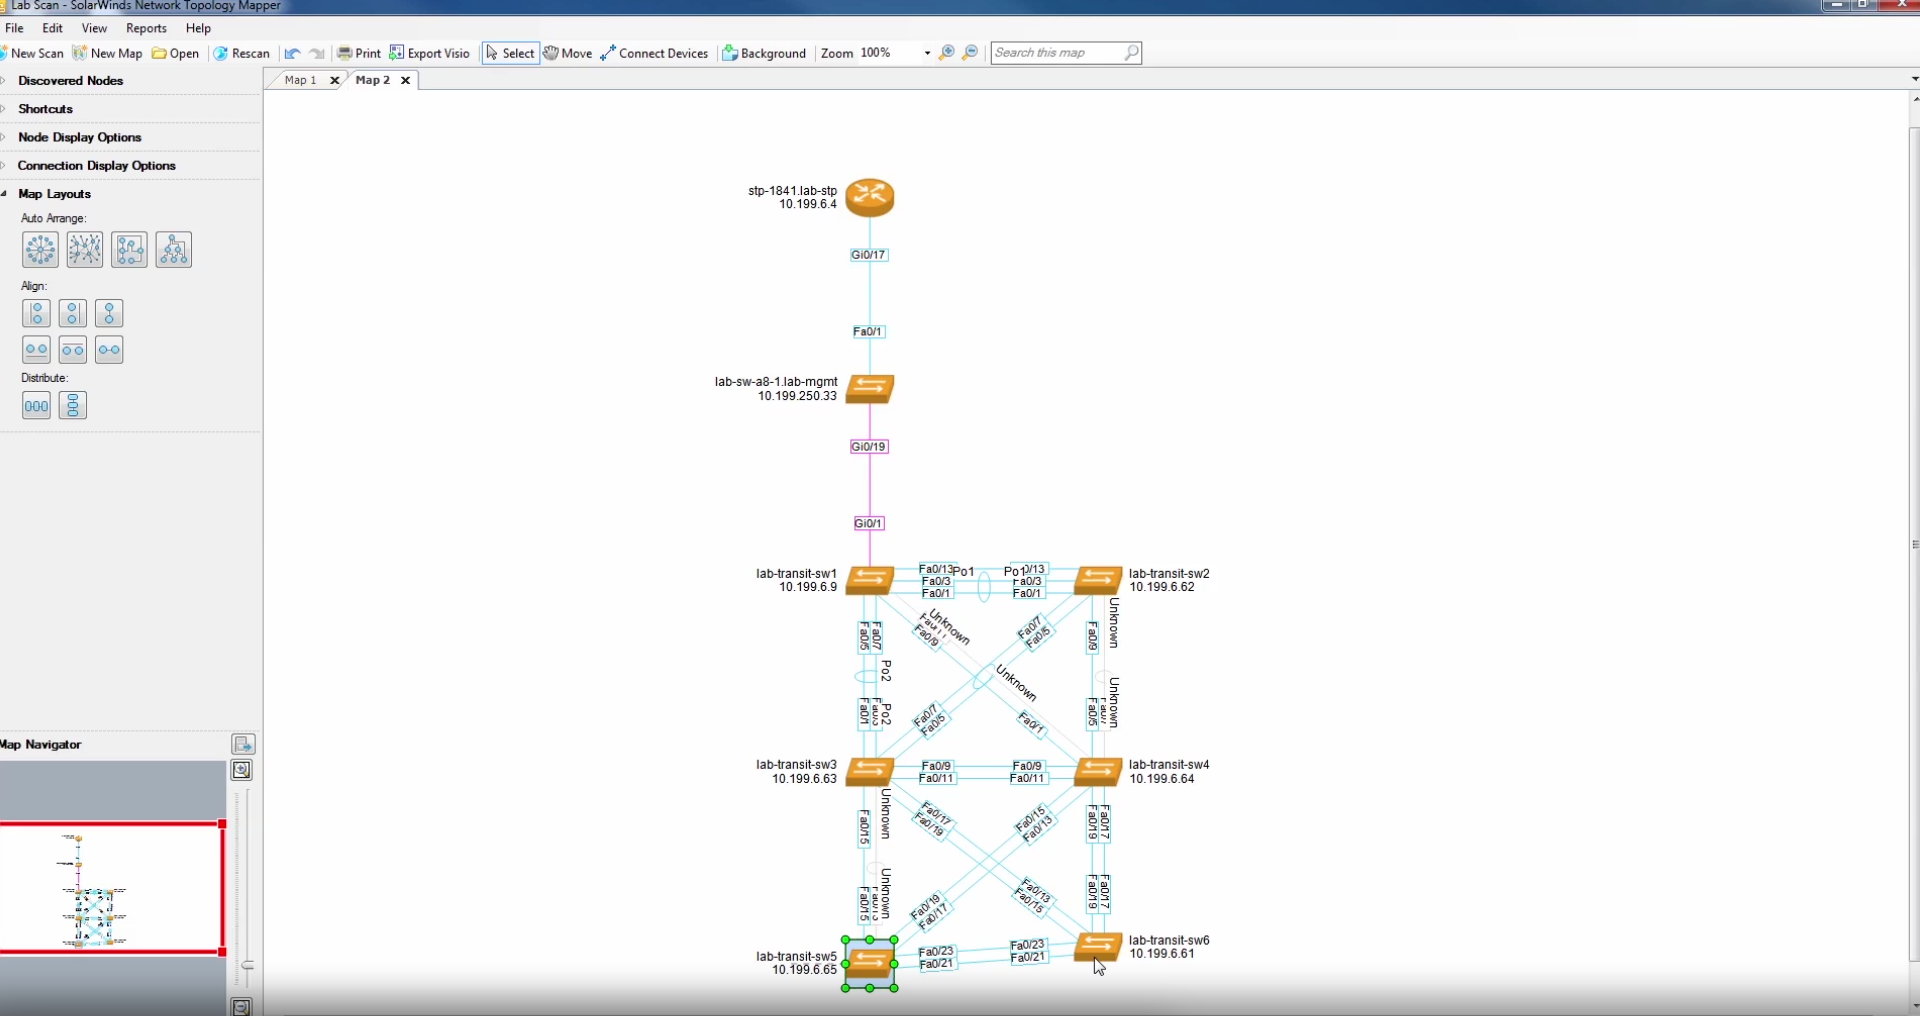
\includegraphics[width=0.8\textwidth]{figures/marco_teorico/solarwinds.png}
    \caption{Ejemplo de diagrama utilizando SolarWinds. \cite{solarwinds}}
    \label{fig:marco:solarwinds}
\end{figure}

\subsection{Comparación de herramientas con el presente trabajo}

En el proceso de investigación del estado del arte se encontraron varias herramientas relacionadas a distintos aspectos del diseño y administración de redes, los más notables de los cuales se enumeraron en las secciones previas. Sin embargo se observó que en general todas las herramientas encontradas atacan otros aspectos del mantenimiento de redes.

M5 Simulator, por ejemplo, permite describir una red y experimentar sobre la misma, pero no deja de ser una simulación, por lo cual pasar de la simulación al mundo físico requiere volver a implementar todo el trabajo realizado en M5 en los equipos reales, de forma manual.

La herramienta que más relación guarda con el presente trabajo es SolarWinds en el sentido que permite acceder a un diagrama que refleje el estado actual de la red. Sin embargo es una herramienta pasiva, no permite modificar la configuración de la red.

Es aquí que la herramienta a desarrollar difiere de las existentes en el mercado: en lugar de ser una herramienta pasiva es activa, el estado definido en el modelo se verá reflejado en la realidad y no al revés.

\section{Sistemas de Manejo de la Configuración} \label{Sistemas de Manejo de la Configuracion}

En cualquier contexto las computadoras cambian continuamente, software es agregado, removido, o actualizado, y sus configuraciones cambian constantemente, lo que se vuelve un problema al tener que manejar decenas o cientos de computadoras al mismo tiempo. De este problema surgen los Sistemas de Manejo de la Configuración.

Existen diferentes herramientas pero todas comparten ciertas características fundamentales \cite{cotton2016what}:

\begin{description}
\item[Aplicación (Enforcement) de configuración:] Es una de las características más importantes, dado que asegura que una computadora siempre este configurada según su especificación, es decir, que se encuentre en su estado deseado en cada momento dado.

Esto significa que el manejador evitará que se produzcan desvíos en la configuración por medio de actualizaciones, o cambios aplicados por terceros (técnicos, trabajadores).

\item[Permite la cooperación:] Facilitan el trabajo en equipo al tener un solo punto de acceso a toda la configuración. 
Esto se hace indispensable a medida que la cantidad de computadoras a configurar aumenta, dado que realizar la configuración de cada una será propenso a fallos, y al mismo tiempo, detectarlos se volverá más dificultoso.

\item[Permite versionado:] La mejor manera de permitir la colaboración en equipo es utilizando un sistema de versionado, una ventaja es que la mayoría de las herramientas en cuestión basan su configuración en archivos de texto, lo que lleva a que la integración con cualquier sistema de versionado sea inmediata, y obteniendo todos sus beneficios ya conocidos.

\item[Permite control de cambios:] Dado que estas herramientas se basan en archivos de texto, y pueden ser versionadas, también se puede realizar sobre ellas un sistema de control de cambios, donde los usuarios envían los cambios a aplicar, se comparan las diferencias, y se lleva a cabo revisión de código antes de aprobar los mismos.
Esto también permite llevar registro de diferentes versiones, en caso de necesitar volver a un estado previo.

\item[Permite la abstracción de los sistemas:] Al tener cierta cantidad de computadoras que mantener, es probable que se tenga que gestionar diferentes sistemas operativos, o al menos, diferentes distribuciones de un mismo sistema. Con herramientas de manejo de la configuración esto deja de ser un problema, ya que se encargarán de abstraer la implementación de configuraciones específicas de los diferentes sistemas o distribuciones.

\end{description}

En las siguientes secciones se presentará una selección de herramientas para el manejo de la configuración. En particular se hará una breve introducción a Puppet, Chef, y Ansible. La elección se basa en que dichas herramientas son las más populares en el área, son de fácil acceso, y poseen un buen nivel de documentación. Además, estas herramientas poseen características similares entre sí, lo que será beneficioso al momento de realizar la implementación, o como consideración para trabajos futuros.

\subsection{Puppet}

Puppet es una herramienta de automatización de configuración de hosts y servidores.
Utiliza un lenguaje propio, declarativo, para definir el estado deseado de los distintos dispositivos.
En sus mejores prácticas utiliza diferentes modelos (rol, perfil, módulo), lo que confiere una gran flexibilidad al momento de configurar nodos.

\begin{figure}[htbp]
    \centering
    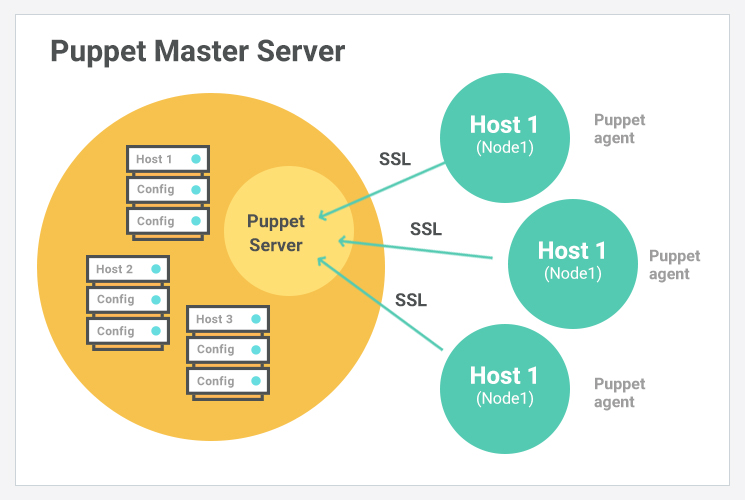
\includegraphics[width=0.75\textwidth]{figures/marco_teorico/puppet_configuration.jpg}
    \caption{Representación del manejo de la configuración a través de Puppet.\cite{chefvspuppet}}
    \label{fig:marco:puppet_configuration}
\end{figure}

\subsection{Chef}
Según su propia definición, Chef es una plataforma de automatización que transforma infraestructura en código. Independientemente de si se opera en servicio Cloud, con servidores locales, o un híbrido, Chef permite automatizar como la infraestructura es configurada, desplegada, y manejada a través de una red, sin importar el tamaño. \cite{chefoverview}

En la Figura \ref{fig:marco:chef_overview} se muestran los diferentes elementos que participan en un ambiente de Chef, incluyendo los nodos, servidores, y estaciones de trabajo. Por otro lado, en la Figura \ref{fig:marco:chef_configuration} se puede ver como se representa el manejo de la configuración en Chef.

\begin{figure}[htbp]
    \centering
    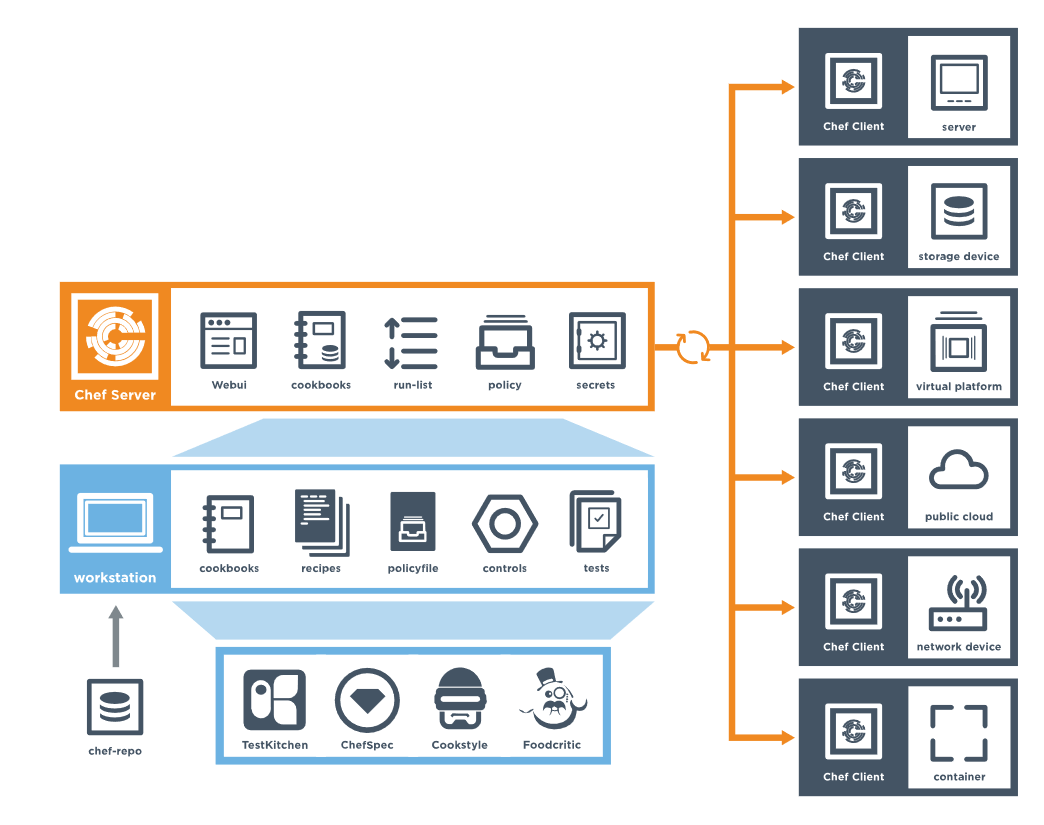
\includegraphics[width=0.75\textwidth]{figures/marco_teorico/chef_overview.png}
    \caption{Elementos presentes en el ambiente de Chef. \cite{chefoverview}}
    \label{fig:marco:chef_overview}
\end{figure}

\begin{figure}[htbp]
    \centering
    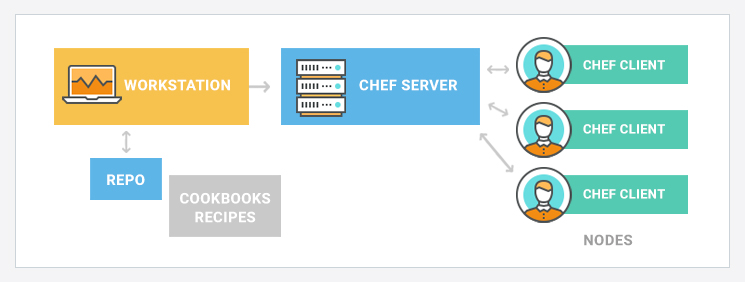
\includegraphics[width=0.75\textwidth]{figures/marco_teorico/chef_configuration.jpg}
    \caption{Representación del manejo de la configuración en Chef. \cite{chefvspuppet}}
    \label{fig:marco:chef_configuration}
\end{figure}

\subsection{Ansible}
Ansible es una herramienta de automatización de IT que permite automatizar diferentes necesidades como aprovisionamiento en servicios cloud, manejo de la configuración, despliegue de aplicaciones, y organización de servicios, entre otros.
Además, es capaz de modelar la infraestructura de IT describiendo como todos los sistemas involucrados se conectan entre sí, en lugar de manejar cada sistema por separado.
Otra característica es que no requiere agentes o una infraestructura de seguridad particular, y utiliza un lenguaje simple como YAML que permite describir los procesos de automatización de una forma similar al inglés. 
En la Figura \ref{fig:marco:ansible_configuration} se puede apreciar el flujo de configuración mediante Playbooks de Ansible, mientras que la Figura \ref{fig:marco:ansible_architecture} muestra un ejemplo de su arquitectura. \cite{ansibleoverview}


\begin{figure}[htbp]
    \centering
    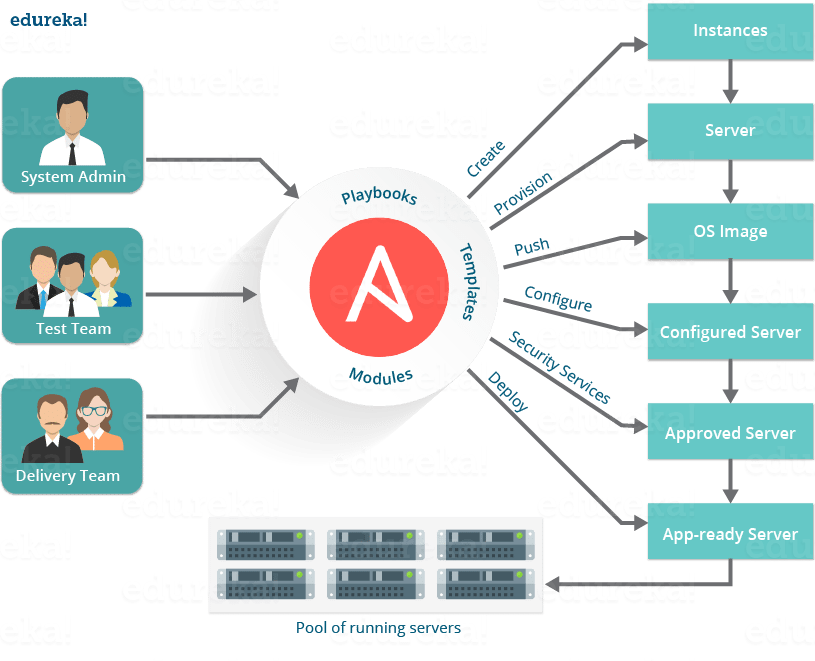
\includegraphics[width=0.7\textwidth]{figures/marco_teorico/ansible_configuration.png}
    \caption{Representación del manejo de configuración de Ansible. \cite{ansiblearchitecture}}
    \label{fig:marco:ansible_configuration}
\end{figure}

\begin{figure}[htbp]
    \centering
    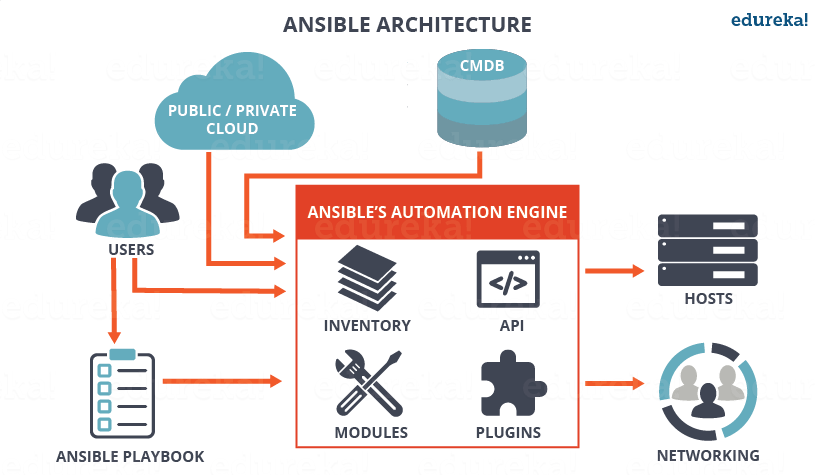
\includegraphics[width=0.7\textwidth]{figures/marco_teorico/ansible_architecture.png}
    \caption{Representación de la arquitectura de Ansible. \cite{ansiblearchitecture}}
    \label{fig:marco:ansible_architecture}
\end{figure}

\section{Model Driven Engineering}
A medida que los sistemas de software han evolucionado, los desarrolladores se han encontrado con nuevos desafíos en el ejercicio de su profesión. Para \cite{clark2015applied} los más importantes son:
\begin{description}
\item[Complejidad] Debido a las necesidades de los negocios y usuarios, los sistemas de software son cada vez más complejos, lo cual trae problemas como tiempos de desarrollo más largos y mayor dificultad de mantener y testear código.
\item[Diversidad] La diversidad de dominios, requerimientos y tecnologías dificulta el proceso de desarrollo de software.
\item[Cambio] El cambio es la constante en los procesos de desarrollo de software: los requerimientos cambian, las tecnologías cambian, las funcionalidades cambian y este cambio dificulta y enlentece el desarrollo.
\end{description}

Es en este contexto que surge el concepto de la Ingeniería Dirigida por Modelos.
La \textit{Ingeniería Dirigida por Modelos} (a partir de ahora MDE, por sus siglas en inglés) es un paradigma en el cual el uso de modelos toma un papel fundamental en todas las actividades ingenieriles \cite{kent2002model}. 
Es así que MDE como disciplina se basa en la idea de que se puede llegar a resolver un problema a partir de la confección de un modelo del mismo.

En una primera instancia sería fácil ver MDE simplemente como generación de software a partir de la creación de un modelo. Esto se denomina Desarrollo Dirigido por Modelos (MDD), pero la disciplina no se limita a esto ya que esta es sólo una de las actividades de la ingeniería, y el uso de modelos puede utilizarse para comprender mejor un problema, para realizar ingeniería inversa, para mejorar la comunicación entre miembros de un equipo o entre equipos, entre otras cosas.

Para entender el proceso de MDE hay que comprender ciertos conceptos fundamentales, como Modelo, Metamodelo y Transformación. A continuación se podrán encontrar definiciones y ejemplos para ayudar a entender claramente dichos conceptos.

\subsection{Modelo}
La Real Academia Española define modelo como \cite{rae2017modelo}:
\begin{description}
\item[4] m. Esquema teórico, generalmente en forma matemática, de un sistema o de una realidad compleja, [...] que se elabora para facilitar su comprensión y el estudio de su comportamiento.
\end{description}

Esta definición da lugar a los dos roles más importantes que cumple un modelo:
\begin{description}
\item[Reducción] Un modelo debe reflejar solamente una selección de las propiedades originales, de modo de enfocarse en los aspectos de interés.
\item[Mapeo] Los modelos son basados en un individuo original, el cual es tomado como prototipo de una categoría de individuos y es abstraído y generalizado en un modelo.
\end{description}
\cite{brambilla2012model}

Entonces se puede decir que un modelo, en el contexto de MDE, es una abstracción simplificada del sistema o entorno que estudia.

\subsection{Metamodelo}

Algunas definiciones de metamodelo lo describen como ``un modelo que define un lenguaje para expresar un modelo''; o como ``un modelo de un lenguaje de modelos''.
Esto quiere decir que un metamodelo describe completamente al lenguaje de modelado en cuestión: su sintaxis concreta, abstracta y semántica \cite{clark2015applied}.

La relación entre metamodelo y modelo, se puede pensar como que un modelo ``Se conforma a'' un metamodelo. \cite{bezivin2005unification}
Por lo tanto, un metamodelo es un modelo de una especificación para el cuál los sistemas estudiados son modelos, en un determinado lenguaje de modelado.
La representación visual de un metamodelo en relación con el modelo y sistema se puede apreciar en la Figura \ref{fig:marco:definicion_metamodelo}. \cite{da2015model}

\begin{figure}[htbp]
    \centering
    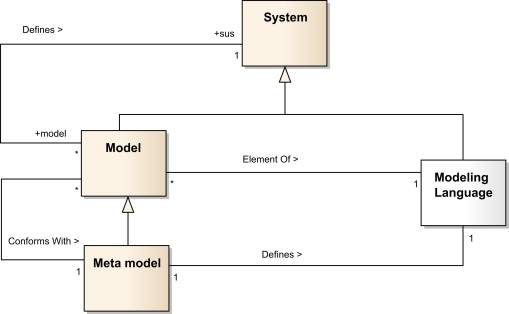
\includegraphics[width=0.75\textwidth]{figures/marco_teorico/metamodelo.jpg}
    \caption{Relación entre metamodelo, modelo y sistema. \cite{da2015model}}
    \label{fig:marco:definicion_metamodelo}
\end{figure}

La relación de un modelo y un metamodelo se puede explicar con tres propiedades de ambos y el lenguaje de modelado. 
Primero, a través de la relación \textit{ElementOf} entre Modelo y Lenguaje de Modelado, un lenguaje de modelado es un conjunto de modelos, (o un modelo es parte de un lenguaje de modelado).
Luego, a través de la relación \textit{Defines} entre Metamodelo y Lenguaje de Modelado, un metamodelo es un modelo de una estructura de lenguaje de modelado (o un lenguaje de modelado es definido por un metamodelo). Finalmente, un metamodelo es un conjunto de modelos o modelo de modelos.

\subsection{Transformación}
Una Transformación de Modelo es el proceso de convertir uno o varios modelos (modelos origen) en un modelo salida (modelo destino/objetivo) del mismo sistema.

Kleppe \cite{kleppe2003mda} definía una transformación como la generación automática de un modelo destino a partir de un modelo origen, en base a una definición. Una definición de transformación es un conjunto de reglas de transformación que en conjunto describen como un modelo del lenguaje origen puede ser transformado en un modelo del lenguaje destino. Por último, una regla de transformación es una descripción de como uno o varios conceptos del lenguaje origen pueden ser transformados en uno o varios conceptos del lenguaje destino.

Las transformaciones también pueden ser aplicadas a múltiples modelos origen, obteniendo múltiples modelos destino, mientras que también se pueden generar transformaciones de modelo a texto \cite{mens2006taxonomy}.

\begin{figure}[htbp]
    \centering
    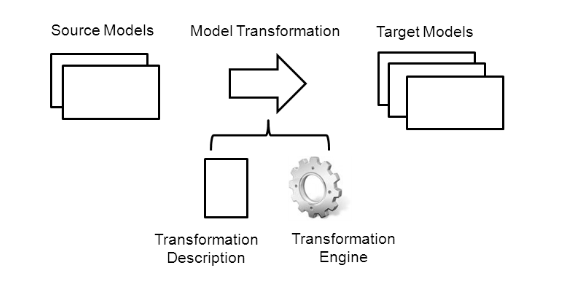
\includegraphics[width=0.8\textwidth]{figures/marco_teorico/model_transformation.png}
    \caption{Componentes de una transformación de modelo. \cite{biehl2010literature}.}
    \label{fig:marco:transformation}
\end{figure}

De la misma forma en que existen transformaciones para obtener modelos de salida a partir de los modelos de origen, conocidas como transformaciones Model-To-Model, también se pueden generar transformaciones de modelo a texto, conocidas como Model-To-Text. El estándar de la transformación de modelo a texto MOF (mof2text) describe como pasar de un modelo a varios artefactos de texto, ya sea código, especificaciones de configuración, reportes, documentos, etc. En esencia, describe cómo obtener una representación en texto a partir de un modelo. Una forma de realizar esta transformación es mediante el uso de plantillas (\textit{templates}), donde el texto que se genera a partir de los modelos se especifica a partir de un conjunto de plantillas de texto, que son parametrizadas con los elementos del modelo en cuestión.

En este enfoque un \textit{template}, o plantilla, especifica un texto con marcadores a rellenar con datos que serán extraídos de los modelos. Estos marcadores son expresiones que se describen utilizando entidades del metamodelo y consultas (\textbf{queries}) para seleccionar y extraer los valores de los modelos. Estos valores son entonces convertidos a texto utilizando como base un lenguaje de expresiones, y alguna librería de manejo de \textit{strings}. \cite{mof_model2text}

\subsection{Diagramas de deployment}
Un Diagrama de \textit{deployment} de UML es una representación del estado actual de la configuración de los nodos y los componentes que se ejecutan en esos nodos. Estos diagramas muestran el hardware del sistema, el software instalado en dicho sistema, y el middleware que conecta las maquinas entre sí. \cite{ambler2018deployment}

En general se utilizan para describir sistemas no triviales, mostrando las diferentes interacciones entre sus componentes, por ejemplo aplicaciones que se ejecutan en varias computadoras, servidores utilizando servicios de firewall, arquitecturas de servicios web, o arquitecturas de sistemas embebidos, mostrando como el hardware y el software funcionan en conjunto.

\begin{figure}[htbp]
    \centering
    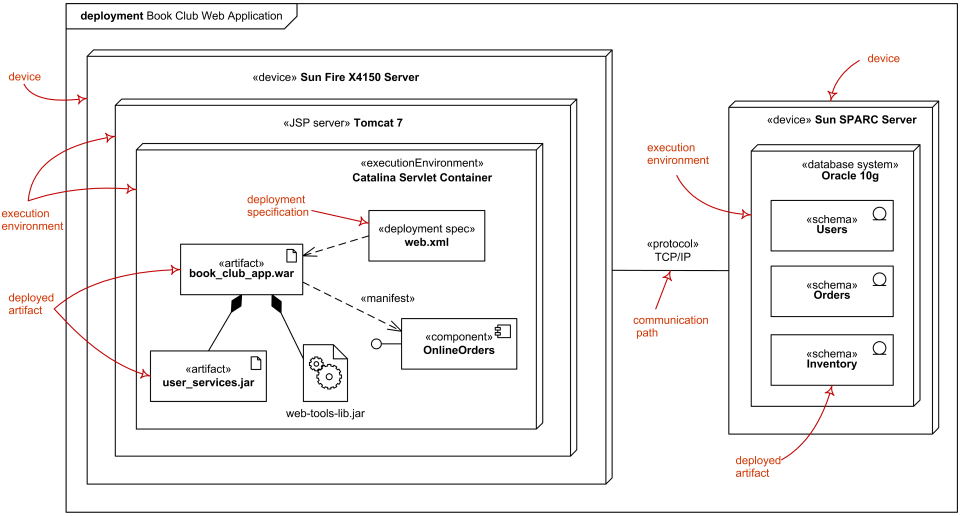
\includegraphics[width=0.8\textwidth]{figures/marco_teorico/deployment-diagram-overview-specification.png}
    \caption{Diagrama de \textit{deployment} a nivel de especificación. \cite{deploymentdiagramoverview}}
    \label{fig:marco:diagram_overview}
\end{figure}

Los diagramas de deployment se suelen crear durante la etapa de implementación en el ciclo de desarrollo, de forma de mostrar cómo se distribuyen los nodos en un sistema distribuido, qué artefactos se encuentran en qué nodos, y los componentes y otros elementos que los artefactos implementan. Los nodos representan dispositivos de hardware como computadoras, sensores, impresoras, y demás dispositivos que puedan soportar un ambiente de ejecución. Al mismo tiempo, las relaciones de deploy (o despliegue) y los enlaces de comunicación modelan las conexiones en el sistema. \cite{ibmdeploymentdiagrams}

\begin{figure}[htbp]
    \centering
    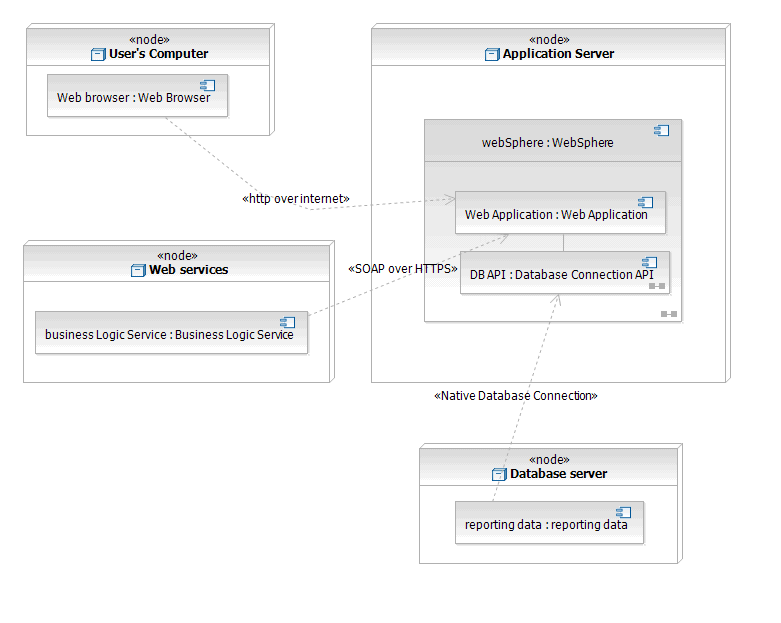
\includegraphics[width=0.8\textwidth]{figures/marco_teorico/deployment-diagram-ibm.png}
    \caption{Ejemplo de un diagrama de deployment. \cite{ibmdeploymentdiagrams}}
    \label{fig:marco:ibmdeploymentdiagram}
\end{figure}

Estos diagramas son útiles para visualizar, especificar, y documentar diferentes tipos de sistemas, algunos ejemplos son los siguientes: \cite{ibmdeploymentdiagrams}
\begin{itemize}
    \item Sistemas embebidos que utilizan hardware que es controlado por señales externas, por ejemplo una pantalla que se controla por cambios de temperatura
    \item Sistemas cliente/servidor que distinguen su interfaz de usuario y los datos persistidos del sistema
    \item Sistemas distribuidos con múltiples servidores y que poseen diferentes versiones de artefactos de software, que pueden ser migrados de nodo a nodo
\end{itemize}

\subsection{Perfiles UML}
Los diagramas de Perfiles en UML brindan un mecanismo genérico de extensión con el fin de personalizar modelos UML para ciertos dominios o plataformas. Estos mecanismos de extensión permiten refinar la semántica estándar de una forma aditiva, lo que evita conflictos con dicha semántica. Los perfiles se definen utilizando Estereotipos (stereotypes), Definiciones de Valores (tagged values definitions), y Restricciones (constrains), los cuales se aplican a elementos específicos del modelo como Clases, Atributos, Operaciones, y Actividades. Un perfil es entonces, una colección de estas extensiones, que en conjunto personalizan UML para un dominio particular \cite{visualparadigm}:
\begin{description}
\item[Stereotypes:]
Los estereotipos permiten incrementar el vocabulario de UML, agregando o creando nuevos elementos del modelo a partir de los existentes, pero que tienen nuevas propiedades específicas acorde a las necesidades particulares del dominio. 

\item[Tagged Values:]
Los valores etiquetados se utilizan para extender las propiedades UML, agregando información adicional en la especificación de un elemento del modelo. Estas se agregan especificando pares de clave-valor a un modelo, donde las claves son los atributos.

\item[Constrains:]
Las restricciones son las propiedades que especifican la semántica o condiciones que se deben cumplir en todo momento. Permiten extender la semántica de construcción de UML agregando nuevos protocolos.
\end{description}

En la Figura \ref{fig:marco:profile_server} se puede ver un ejemplo de como se define un perfil UML.
En este caso se quiere definir el elemento Servers, por lo que extiende la metaclase Device con el estereotipo de dicho nombre, de esta forma se tendrá el elemento Server, que tendrá el comportamiento de la metaclase Device, y además poseerá los atributos que fueron definidos en dicho estereotipo: Vendor, CPU, y Memory.

\begin{figure}[htbp]
    \centering
    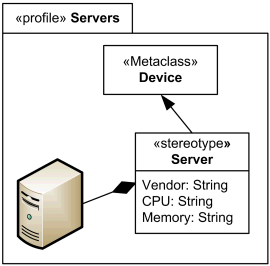
\includegraphics[width=0.5\textwidth]{figures/marco_teorico/profile-servers.png}
    \caption{Ejemplo de perfil UML Servers. \cite{umlprofile}}
    \label{fig:marco:profile_server}
\end{figure}

El perfil podría utilizar todos, o parte de otros perfiles ya definidos, además, multiples perfiles pueden ser aplicados a un mismo modelo.

\section{Herramientas de MDE}
\subsection{Eclipse Modeling Framework}
Eclipse Modeling Framework (EMF) es un framework de modelado y generación de código diseñado para construir herramientas y otras aplicaciones basadas en un modelo de datos estructurado.  
A partir de una especificación de modelo en XMI, permite producir un conjunto de clases java para el modelo, así como un conjunto de clases adaptador que permiten visualizar, y utilizar comandos para editar el modelo. EMF también provee un editor básico para trabajar sobre el modelo y las clases de java.

En particular, EMF Core es un estándar para modelado de datos, por lo que muchas tecnologías y frameworks se basan en dicho estándar. 
EMF Core consiste de tres partes fundamentales \cite{steinberg2008emf}:
\begin{description}
\item[EMF:] Incluye un meta modelo (Ecore) para describir modelos y soporte en tiempo de ejecución para los modelos, incluyendo notificación de cambios, persistencia con serialización XML, y una API para manejar objetos EMF.

\item[EMF.Edit:] Incluye clases genéricas reusables para construir editores de modelos EMF.

\item[EMF.Codegen:] La generación de código de EMF permite generar cualquier elemento necesario para construir un editor de modelos EMF completo. Incluye una interfaz gráfica (GUI) donde se pueden especificar opciones de generación, y llamar a los generadores.
\end{description}

\subsection{Papyrus}
Papyrus es una herramienta de modelado gráfico para UML2 basado en Eclipse. Al ser una herramienta de MDE, provee generación de código y permite interacción o conexión con herramientas externas de forma que los modelos sean los artefactos principales del proceso de desarrollo.
Papyrus también posee muchas características para diseño de Domain Specific Modeling Languages (DSMLs) utilizando el concepto de perfiles UML, y por defecto incluye un conjunto de plug-ins de extensiones (perfiles UML 2) predefinidos dedicados a aplicaciones embebidas en tiempo real, como los estándares OMG (Object Management Group) SysML, MARTE, CCM, y LwCCM.

Algunas de las características de Papyrus descriptas en su propia página web, son representadas en la Figura \ref{fig:marco:papyrus_editor}.

\begin{figure}[htbp]
    \centering
    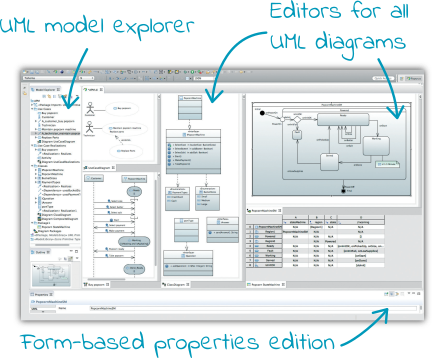
\includegraphics[width=0.8\textwidth]{figures/marco_teorico/papyrus-features.png}
    \caption{Características del editor de Papyrus. \cite{papyrus}}
    \label{fig:marco:papyrus_editor}
\end{figure}

\subsection{Acceleo}
Acceleo es una herramienta de generación de código que implementa la especificación del estándar para transformación de modelo a texto MOF Model to Text Languange del Object Management Group (OMG). Algunas de las características que el IDE provee a los desarrolladores son: sintaxis simple, generación de código eficiente, y herramientas avanzadas equivalentes a las de Java Development Tools. Su propósito es el de asistir al desarrollador durante el ciclo de vida de sus generadores de código. \cite{acceleo}

\begin{figure}[htbp]
    \centering
    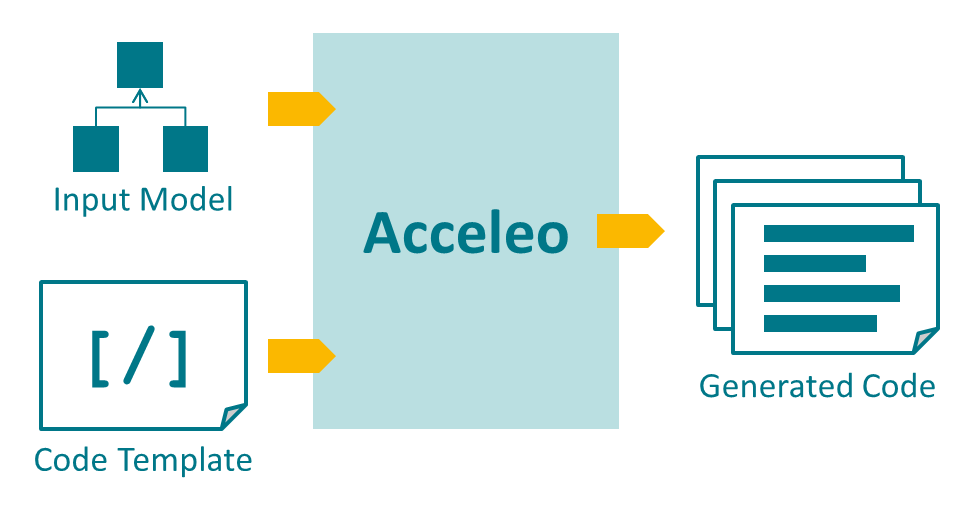
\includegraphics[width=0.8\textwidth]{figures/marco_teorico/acceleo.png}
    \caption{Proceso de transformación de Acceleo. \cite{acceleo}}
    \label{fig:marco:acceleo_transformation}
\end{figure}

\subsection{ATL}
ATL (ATL Transformation Language) es un lenguaje y herramienta de transformación de modelos. Para MDE, ATL provee formas de producir un conjunto de modelos destino, a partir de un conjunto de modelos origen. Una transformación de ATL se compone de reglas que definen cómo los elementos de los modelos de origen se obtienen y navegan para crear e inicializar los elementos de los modelos destino. \cite{atl}

Una transformación de modelo a modelo se corresponderá con un módulo ATL. Estos módulos se encargan de definir dicha transformación, y están compuestos por los siguientes elementos \cite{atloverview}:

\begin{itemize}
    \item una sección \textbf{header} (encabezado) que define algunos atributos relativos al módulo de la transformación
    \item una sección opcional \textbf{import} que permite importar librerías existentes de ATL
    \item un conjunto de \textbf{helpers} que se pueden ver como el equivalente de ATL a los métodos de Java
    \item un conjunto de \textbf{reglas} que definen cómo los modelos de destino serán generados a partir de los modelos de origen
\end{itemize}

\section{MDE en redes de computadoras}
\subsection{MDE en sensores de red inalámbricos}
El artículo \cite{essaadi2017mde} presenta un enfoque de ingeniería dirigida por modelos para llevar a cabo el desarrollo de aplicaciones de Sensores de Red Inalámbricos. Es necesario manejar la complejidad en aumento de estos sistemas, y se enfoca en aumentar la flexibilidad y reusabilidad del diseño.
Los tres niveles de abstracción definidos permiten construir: modelos de dominio específico, descripciones de arquitectura basada en componentes, y modelos específicos a la plataforma. También se definen transformaciones entre estos tres niveles.

\subsection{YANG}
YANG es un lenguaje de modelado utilizado para modelar configuración y estado de datos utilizados por el protocolo de configuración de redes NETCONF (Network Configuration Protocol).
Los modelos de datos definidos en un modulo de YANG se representan en XML, y las operaciones NETCONF se utilizan para manipular los datos.
A su vez, cada módulo define la jerarquía de datos que pueden ser utilizados para operaciones basadas en dicho protocolo, incluyendo configuración, estado de datos, llamadas a procedimientos remotos (RPCs), y notificaciones. Esto permite una descripción completa de todos los datos enviados entre un cliente y servidor NETCONF. \cite{bjorklund2010yang}

\subsection{Metamodelo para Configuraciones en Dispositivos de Redes}
En la tesis con nombre Metamodelo para Configuraciones en Dispositivos de Redes como Estándar Soportado en la Ingeniería Dirigida por Modelos, 
se busca desarrollar una herramienta que estandarice y facilite la administración de redes de forma de poder configurar cualquier protocolo independientemente del proveedor, para lo que se desarrolló un metamodelo que permita generar dicha herramienta.

En este trabajo se describe el metamodelo, desarrollando un DSL para la configuración de dispositivos de red, sin considerar la configuración de computadoras o servidores. Para esto se definen los componentes necesarios, que serán implementados mediante el DSL. En primer lugar se tienen los componentes Router y Switch, asociados a un componente de Interfaz, luego se definen los componentes Brand (Marca) y Protocol (Protocolo), y finalmente se tiene el componente de Configuración que une todos los conceptos.  En la Figura \ref{fig:marco:eclassdiagram} se puede ver el diagrama de clases utilizado para dicha implementación, mientras que en la Figura \ref{fig:marco:routerconfigurationexample} se tiene un ejemplo del resultado de un archivo de configuración para un router.
Finalmente, no define ni busca integrarse con otra herramienta, sino que propone las bases con el metamodelo definido, que estandarizará y facilitará la configuración de redes. \cite{higuerametamodelo}

\begin{figure}[htbp]
    \centering
    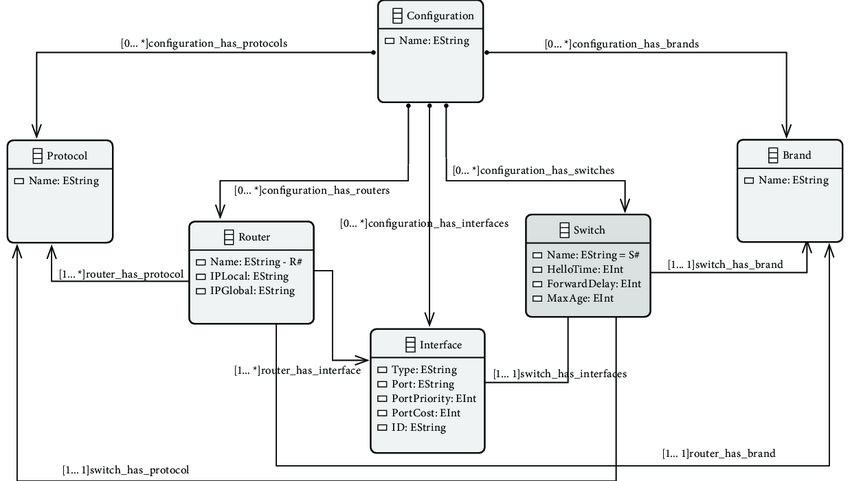
\includegraphics[width=0.8\textwidth]{figures/marco_teorico/diagrama_eclases.png}
    \caption{Diagrama de Eclases del modelo de dominio. \cite{higuerametamodelo}}
    \label{fig:marco:eclassdiagram}
\end{figure}

\begin{figure}[htbp]
    \centering
    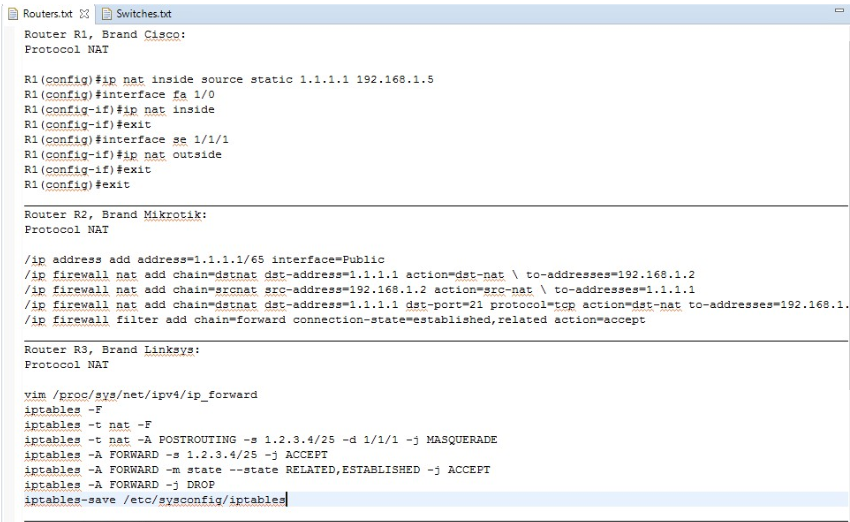
\includegraphics[width=\textwidth]{figures/marco_teorico/salida_router.png}
    \caption{Ejemplo de salida para la configuración de routers. \cite{higuerametamodelo}}
    \label{fig:marco:routerconfigurationexample}
\end{figure}


%%% Local Variables:
%%% TeX-master: "../main"
%%% End:
